\section{Several ways to generate a counterfactual explanation}
To avoid overloaded notations and unify the symbols, only one meaning is assigned to one letter, the notations are:
%统一字母代号:
% K是特征,feature channel
% N是样本 instances
% D是什么?
% i 分类类别

{\centering
\begin{tabular}{|c|l|}
\hline
   notation&meaning\\
  \hline
  % after \\: \hline or \cline{col1-col2} \cline{col3-col4} ...
  k & feature, and K is the total number of feature \\
  m,n & arbitrary instances, and N is the total number of instances \\
  i,j & class label\\
  \hline
  \textbf{x} & input data\\
  \textbf{c} & counterfactual example\\
  \hline
\end{tabular}}
\subsection{generation by loss function}\label{sec:lossFunc}
CF explanation doesn't require to understand the internal work principle of a model, instead focusing on which kind of minimal perturbation in the data subject will leads to a different classification result. Therefore, the search of a an appropriate CF example is boiled down to an optimizing problem with at least two requirements: (1.) classified as the counter class, and (2.) still similar to the original data with only necessary modifications. \cite{watcher2017} has proposed the following formulation, which becomes the basis of the following research:
\begin{equation}\label{eq:watcher}
  \textbf{c}=\arg\min_{\textbf{c}}trgtloss(f(\textbf{c}),y)+d(\textbf{x,c})
\end{equation}
where \textbf{x} is the original data, y is the target data class, \textbf{c} is the generated counterfactual data, and f is the model so that f(\textbf{c}) is the new prediction of the model, i.e. the new class. The first part of the formula encourages a different class, while the second part penalizes large distances away from the original data.

To facilitate equation \ref{eq:watcher} one need to define it in detail, namely how to define "loss" and "distance", which has a significant impact on final results. Another main contribution of \cite{watcher2017} is to define distance as \emph{$L_1$} norm divided by MAD (median absolute deviation):
\begin{equation}\label{eq:distMAD}
  dist = \sum_{k=1}^{K}\frac{|\textbf{x-c}|}{MAD_k}
\end{equation}
where MAD is defined for every feature k over the whole points set P:
\begin{equation}\label{eq:MAD}
  MAD_k=median_{i\in P}(|{X_{i,k}}-median_{j\in P}(X_{j,k})|)
\end{equation}
The \emph{$L_1$} norm in equation \ref{eq:distMAD} prone to generate zero entries, which ensures a sparse optimizing result. Normalising the norm is important as well, otherwise big range data would have heavy weights. Here MAD turns out to outperform standard deviation, because it cooperates with \emph{$L_1$} norm better, and generates a even more sparse result.

Sometimes data may contain categorical features (e.g. occupation, gender\dots), it is counter-intuitive to define "distance" for these features. A simple matching distance is used here, where distance 1 is assigned to value changes and 0 if the value remains unchanged.
\begin{equation}\label{eq:distCate}
  dist\_cat(\textbf{c,x})=\sum_{k=1}^{K_{cat}}\mathbb{I}(c^k\neq x^k)
\end{equation}
Combining equation \ref{eq:distMAD} and \ref{eq:distCate} weighted by the number of continuous and categorical features, the most common used distance metric is shown as following:
\begin{equation}\label{eq:distCombined}
  d(\textbf{x,c})=\frac{1}{K_{con}}\sum_{k=1}^{K_{con}}\frac{|\textbf{x-c}|}{MAD_k}
  +\frac{1}{K_{cat}}\sum_{k=1}^{K_{cat}}\mathbb{I}(\textbf c^k
  \neq \textbf x^k)
\end{equation}

Choosing an appropriate loss term for the target class is of equal importance. Without loss of generality, in this article we choose 0 as the original class label, and 1 for the desired label. Note that the prediction of the model f(\textbf{c}) is a continuous value between 0 and 1 for binary classification. One of the choices of the target loss term is the \emph{$L_2$} norm $(f(\textbf{c})-y)^2$. \cite{DiCE} argues that a valid counterfactual suffices if it bypasses the classification threshold of the model (typically 0.5), but the \emph{$L_2$} norm always prefer the extreme value 1. The underlying issue is that counterfactuals, unless predicted exactly as 1, still receives penalty even if it is classified correctly. A better choice is the hinge-loss:
\begin{equation}\label{eq:hingeloss}
  hinge\_trgtloss=\max(0,1-logit(f(\textbf{c})))
\end{equation}
\begin{figure}
  \centering
  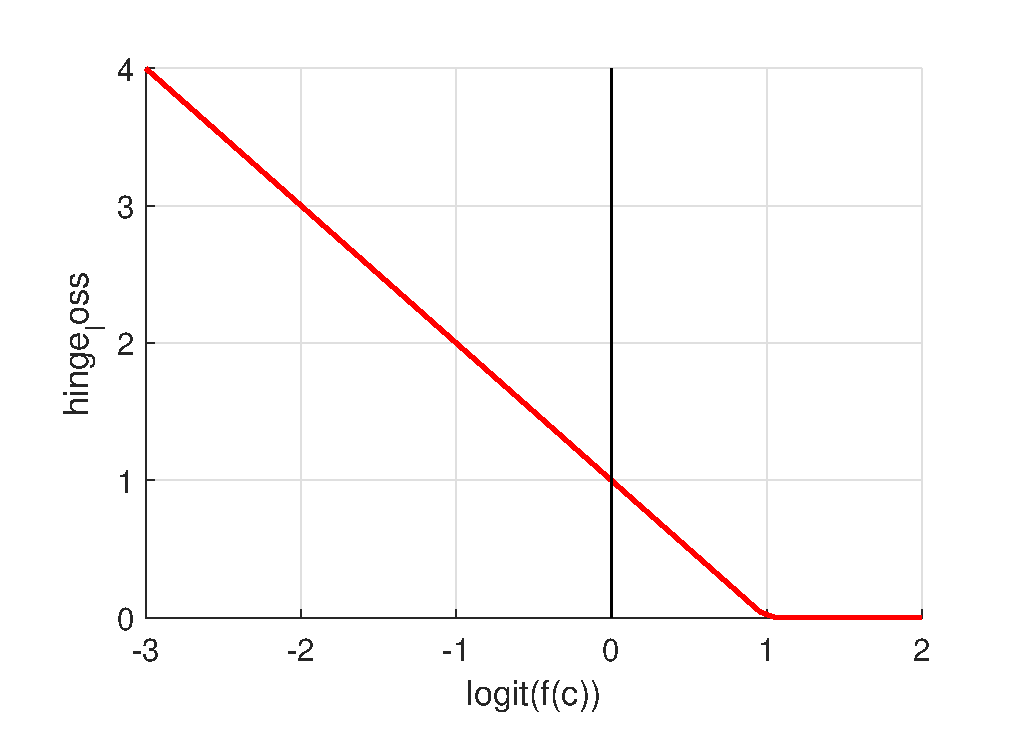
\includegraphics[width=0.5\textwidth]{hingeloss.eps}
  \caption{the hinge loss penalize wrong classification heavily, correct one near the boundary slightly and has no effect above a certain threshold}\label{fig:hingeloss}
\end{figure}
where \emph{logit(f(\textbf{c}))} is the final activation before entering a sigmoid/softmax output layer. This loss function, however, requires internal logits of the model, therefore not available under a "black-box" situation.

So far the equations are derived for a binary classification problem, where a "why A not $\neg${A}" or "why A not B" question is raised. For n-ary classification, where the prediction output is a n-length vector, \cite{prototype} mentioned the following formula:
\begin{equation}\label{eq:lossPred}
  predloss=\max([f(\textbf{c})]_{i=i_0}-\max_{i\neq i_0}[f(\textbf{c})]_i),-\kappa)
\end{equation}
where $i_0=\arg\max f(\textbf{x})$ is the original data label, and $[f(\textbf{c})]_i$ is the i-th class prediction probability. This loss function gives a negative value if the predicted class is different than the original class, and $-\kappa < 0$ caps the negative value.

After fill the framework equation \ref{eq:watcher} with details, it is already able to generate counterfactuals. Some additional terms are introduced for better performance.
\subsubsection{add a diversity term}
As mentioned in the introduction, providing a diverse list of counterfactuals to choose from could be more helpful rather than one single "most feasible" solution. A valuable CF algorithm is able to generate multiple CF instances that are distinct from each other. Meanwhile, the counterfactuals should still proximate the original input. CFs that reach diversity by changes in numerous features, or too fierce changes, are considered inappropriate. This is realized by adding a specific diversity loss term to the loss function. \cite{DiCE} proposed to use the determinant of a kernel matrix as the diversity metric for n counterfactuals:
\begin{equation}\label{eq:dpp}
  dpp\_diversity(\mathbf{c_1,\dots,c_n})=\det(\mathbf{K}),\ \mathbf{K}_{i,j}=\frac{1}{1+dist(\mathbf{c_i,c_j})}
\end{equation}
%TODO: DPP的数学特征? OK
This matrix is named after a widely adopted sampling method DPP (determinantal point processes). DPP focuses on sampling diverse contents and avoiding redundancy. In DPP context the matrix shown above is referred as a marginal kernel. Note that marginal kernel is a mathematical definition, and this specific form is not the only way to construct it. A key rule is, the more similar the chosen candidates are, the smaller the determinant of the kernel matrix will be. For detailed mathematical derivation the readers are redirected to the second chapter of \cite{kulesza2011dpp}, here only an intuitional example is given.
\paragraph{dpp marginal kernel}
A DPP samples a subset \emph{A} of a discrete set \textbf{Y} with the following rule:
\begin{equation}\label{er:dpp}
  \mathcal{P}(A\subset\textbf{Y})=\det(K_A)
\end{equation}
which means the probability of choosing a certain subset equals to the minor of matrix \emph{K}, and \emph{K} is constructed by some relation of all elements in the complete set \textbf{Y}. Considering the simplest case with only two candidates \emph{i,j} in the subset, the possibility is:
\begin{equation}\label{eq:dpp1}
\begin{split}
  \mathcal{P}(i\in\textbf{Y})&=\det(K_{ii})=K_{ii}
\\
  \mathcal{P}(i,j\in\textbf{Y})&=\det\begin{pmatrix}
                                       K_{ii} & K_{ij} \\
                                       K_{ji} & K_{jj}
                                     \end{pmatrix}
                                      \\&=K_{ii}K_{jj}-K_{ij}K_{ji}
                                      \\&=\mathcal{P}(i\in\textbf{Y})\mathcal{P}(j\in\textbf{Y})-K_{ij}^2
\end{split}
\end{equation}
move a term to the left side we obtain the following equation, on the left side is exactly the definition of covariance:
\begin{equation}\label{eq:dpp2}
\begin{split}
  \mathcal{P}(i,j\in\textbf{Y})-\mathcal{P}(i\in\textbf{Y})\mathcal{P}(j\in\textbf{Y})=-K_{ij}^2
  \\\equiv Cov(i,j)=-K_{ij}^2
  \end{split}
\end{equation}
therefore, the possibility to choose a subset with two candidates equals the product of their independent possibility (marginal possibility) plus their (negative) covariance. The more relevant two candidates are, the higher $K_{ij}$ value is. When $\mathcal{P}(i),\mathcal{P}(j)$ are constants, a higher $K_{ij}$ value leads to a greater negative value of $\mathcal{P}(i,j)$ (i.e. the determinant of the matrix), which means a lower co-occurring chance. For 3-order matrix and higher, the explanation is no longer so intuitive.

Since multiple CFs are generated instead of only one, the basic formula needs to be modified before the diversity term is appended. The target loss and distance terms are averaged among all instances, a negative symbol is attached to diversity term because of the $\arg\min$ condition:
\begin{equation}\label{eq:DiCe}
\begin{split}
  \mathbf{C(x)}=\mathop{\arg\min}_{\mathbf{c_1,\dots,c_N}}&\frac{1}{N}\sum_{n=1}^{N}trgtloss(f(\mathbf{c_n}),y)
  +\frac{1}{N}\sum_{n=1}^{N}dist(\mathbf{c_n,x})
  \\&-dpp\_diversity(\mathbf{c_1,\dots,c_N})
\end{split}
\end{equation}
%TODO: Proximity, Sparsity 和Diversity的关系?
\subsubsection{add an interpretability term}
During the search of a CF example, it is equally important to demonstrate that the example is representable for the counter class, otherwise it is neither informative nor reasonable. For example, a user may want to change his occupation for better credits, but change the occupation to "professor" with educational background unchanged as "middle school" does not seem like a plausible answer. One trivial solution, as mentioned in the conclusion of \cite{bertossi2020asp}, is to abandon data generation, and only choose a closest case with the opposite label from a data bank.

To handle with this issue, \cite{prototype} proposed a prototype loss term, to measure the distance from the generated CF to other CF classes in latent layer. For each CF class \emph{i}, the algorithm firstly picks out the N nearest neighbours of the input that are classified as \emph{i}, then feeds them through an encoder and averages the output as the prototype of this CF class.
\begin{equation}\label{eq:prototype}
  proto_i=\frac{1}{N}\sum_{n=1}^{N}\mathbf{ENC}(\mathbf{x_n^i})
\end{equation}
Among all prototypes, the closest one to the input is chosen as the "guidance" for optimization:
\begin{equation}\label{eq:closestProto}
  j = {\arg\min}_{i\neq f(\textbf{x})}||\mathbf{ENC}(\textbf{x})-proto_i||_2
\end{equation}
The prototype loss term is defined as following:
\begin{equation}\label{eq:protoloss}
  prttyploss=||\mathbf{ENC}(\textbf{c})-proto_j||_2^2
\end{equation}
With the guidance of prototype, the perturbation is oriented to one chosen CF class rather than random search. The encoder used here could be any external known model, therefore requiring no internal information of the "black-box" model in question. We see that the closest target class to the input is chosen for a multiple classification task, this however could be revised for binary classification by explicitly choosing a target class.

\cite{prototype} furthermore shows that with the help of prototype loss term in searching, the target loss term could be dropped for improving efficiency. Generation methods based on loss function requires the gradient chain to know the optimization direction in next step. Unfortunately, as CF algorithms are often applied to "black-box" models, only the input data and the final prediction are available, the internal gradients are lost. Therefore, in order to measure the effect of a single perturbation of a feature \emph{k} on the final prediction, the gradient has to be approximated numerically by:
\begin{equation}\label{eq:gradientNumerical}
  \frac{\partial f_{pred}}{\partial x_k}\approx\frac{f_{pred}(x+\epsilon_k)-f_{pred}(x-\epsilon_k)}{2\epsilon}
\end{equation}
and this needs to be done on each feature in both directions for each gradient step, which results in numerous computation. For example, for a $28\times28$ MNIST image, the algorithm needs to call the model for $28\cdot28\cdot2$ times. Before, such numerous computation is still tolerated, because the target loss term ${trgtloss(f(\textbf{c}),y)}$ is the only roll that leads the generation to the target label. However, now the prototype loss term is also able to play the same guidance roll, and requires no internal information. The addition of ${prttyploss}$ significantly reduces both time and iterations about 80\%. Moreover, the generated CFs are more representative for one of the CF classes, as shown in figure \ref{fig:protoresult}. 
\begin{figure}
  \centering
  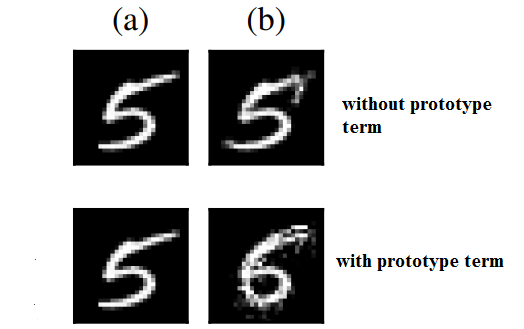
\includegraphics[width=0.5\textwidth]{proto.PNG}
  \caption{(a) column is the input data and (b) column is the CF output. In the first row, input class is 5 and CF class is 3. Second row, input class is 5 and CF class is 6. The addition of the prototype loss term generates a more interpretable CF.  
  }
  \label{fig:protoresult}
\end{figure}

The target loss term, in contrast, increases the time and results in a less interpretable CF, hence becomes a drawback in the whole formula and could be removed.
